\documentclass{article}
\usepackage{listings, graphicx, fontspec}
\lstset{language=Python}

\setmainfont{YanoneKaffeesatz-Light}

\begin{document}

\begin{titlepage}

\begin{flushright}
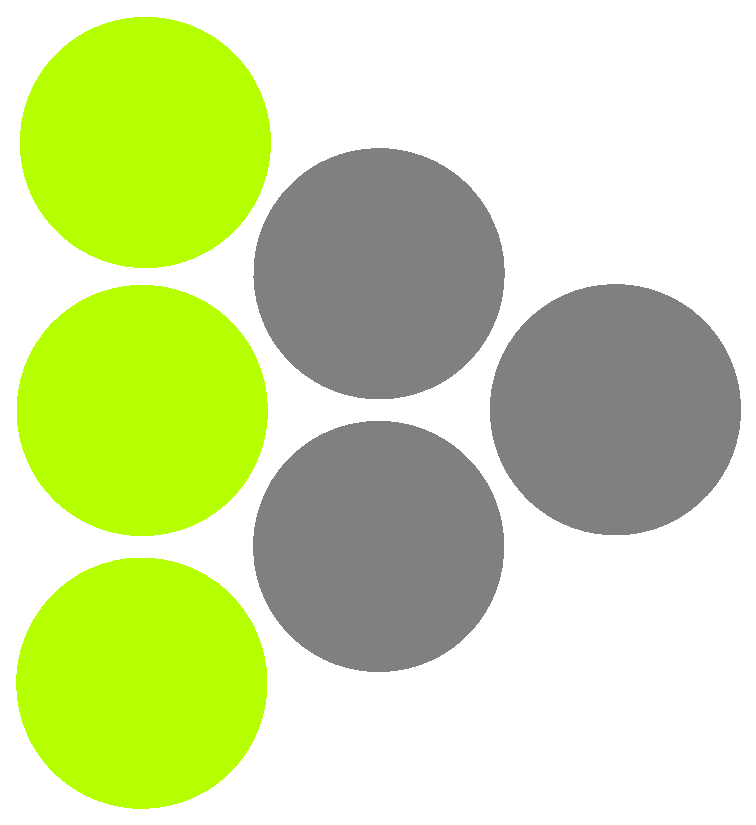
\includegraphics[scale=0.4]{../images/logo_ecidadania.eps}\\
\end{flushright}

\begin{flushleft}

\includegraphics[scale=0.55]{../images/logo_name.eps}\\
\end{flushleft}

\begin{center}

\large Citizen participation platform based on web services\\[0.3cm]

\textsc{\Large strategy report}\\[1cm]
{\normalsize \today}

\end{center}

\begin{minipage}{0.5\textwidth}
\begin{flushleft}
\emph{Author:}\\
Oscar \textsc{Carballal Prego} \texttt{<info@oscarcp.com>}
\end{flushleft}
\end{minipage}
\begin{minipage}{0.5\textwidth}
\begin{flushright}
\emph{Company:}\\
Cidadania Sociedad Cooperativa\\
\texttt{<cidadania@cidadania.coop>}
\end{flushright}
\end{minipage}
\end{titlepage}

\newpage

\begin{abstract}
This paper represents the work for a citizen participation project through the web (E-CIDADANIA) which will allow the users participate with their proposals and debate the proposals before they get to another place.

e-cidadania is an extensible, modular and completely customizable application based on web standards and open-source. There are a number of applications developed as the basis of the project but its not limited to that. There is anspecial emphasis on the social networks and compatibility with all the current popular services on the web like Facebook, Twitter, OpenID, etc. which will allow the user to easily participate when needed.

There are also some middleware software that allows administrators to check the data of the users.
\end{abstract}
\newpage

\tableofcontents
\newpage

\section{Introduction}
Currently is very common to find a e-democracy project running for some kind of reason. But based on existing experiencies, we know that all those platforms are left abandoned after a while (one or two years).

The e-cidadania project implements all the best ideas around the e-democracy and tries to keep the people participating, because the participation is not limited to the final voting. Instead there are a lot of previous reunions to put in common the proposals and other stuff.

The end purpose of this project is to develop a pcitizen participation application for digital democracy that doesn\'t end in the trash after one year of life.

\section{Architectural model}
In this citizen participation platform the users will have access to the system in a lot of ways: debates, proposals, wiki, documents, votes, etc. The applications can be configured to do various ways of authentication, also the security leves vary depending the scenario. Some parts of the system are accesible as an anonymous user.

\begin{itemize}
\item {\bf Flexibility configuring the enviroment}. The environment must be adaptable for every place.
\item {\bf Multiple sites per instance}. The platform must support multime sites per server instance to avoid saturation.
\item {\bf Multiple authentication methods}. LDAP, DB users, OpenID.
\item {\bf Modular}. The system must be modular so at any time it can be updated with new applications or enhancements.
\item {\bf Social}. The application must be seemingly integrated with current social sites like Facebook, Twitter, Identi.ca, Digg, etc.
\end{itemize}

\newpage

\begin{figure}
	\centering
		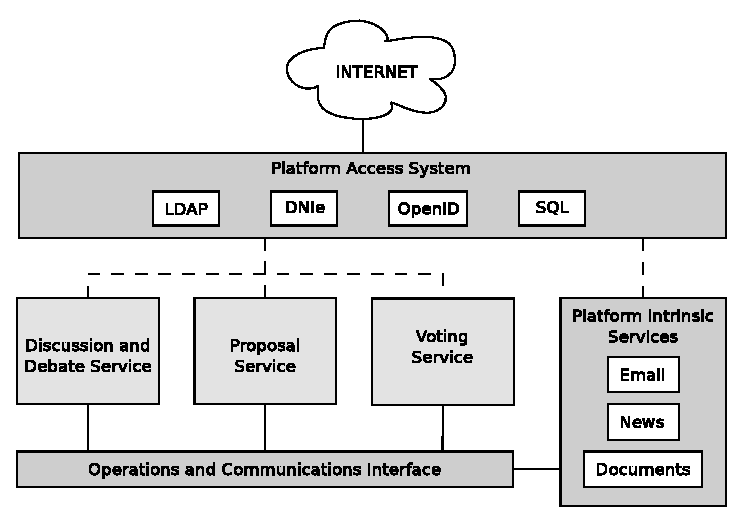
\includegraphics[scale=1]{../images/architecture.eps}\\
	\caption{Platform Architecture of e-cidadania}

\end{figure}

\section{Definition of e-cidadania platform}
To develop the e-cidadania platform we chose to use web services and base it on Django framework.

\subsection{Applications supported by e-cidadania}
The platform will come with some applications built-in to start working, even if later there are needs to implemtn more applications.

\begin{itemize}
\item {\bf Debate forums}. The debate forums are in a bidimensional way
\item {\bf News and notice boards}. Very much like a blog.
\item {\bf Proposals}. Everyone can make proposals.
\item {\bf Participative budgets}.
\end{itemize}

\subsection{Definition of web services}

{\bf Census}. This application handles all the operation related to users and census for every community scenario.
\end{document}
